\documentclass{article}
\usepackage[utf8]{inputenc}
\usepackage{amsmath,amsbsy,amssymb}
\usepackage[english]{babel}
\usepackage{xcolor}
\usepackage{rotating}
\usepackage{xcolor,cancel}
\usepackage{amsmath}


\title{TDycore Test Problems}
\author{Glenn Hammond}
\date{\today}

\newcommand{\eq}{\ =\ }
\newcommand{\p}{{\partial}}
\newcommand{\im}{{\rm im}}
\newcommand{\m}{{\rm m}}
\newcommand{\A}{{\mathcal A}}
\newcommand{\bnabla}{\boldsymbol{\nabla}}
\newcommand{\bc}{\boldsymbol{c}}
\newcommand{\bnu}{\boldsymbol{\nu}}
\newcommand{\bq}{\boldsymbol{q}}
\newcommand{\bn}{\boldsymbol{n}}
\newcommand{\Bf}{\boldsymbol{f}}
\newcommand{\bK}{\boldsymbol{K}}
\newcommand{\bG}{\boldsymbol{G}}
\newcommand{\bA}{\boldsymbol{A}}
\newcommand{\bB}{\boldsymbol{B}}
\newcommand{\bJ}{\boldsymbol{J}}
\newcommand{\bv}{\boldsymbol{v}}
\newcommand{\bx}{\boldsymbol{x}}
\newcommand{\bbx}{\boldsymbol{\bar{x}}}

\def\EQ#1\EN{\begin{equation}#1\end{equation}}
\def\BA#1\EA{\begin{align}#1\end{align}}
\def\BS#1\ES{\begin{split}#1\end{split}}
\def\EQA#1\ENA{\begin{eqnarray}#1\end{eqnarray}}

\usepackage{natbib}
\bibliographystyle{abbrvnat}

%\addbibresource{references.bib}


\begin{document}

\maketitle

\section{Steady State Groundwater Flow Equation}
The governing equation for steady state groundwater flow is
\EQ
\nabla \cdot \frac{k\rho}{\mu} \nabla p = 0
\EN
with intrinsic permeability $k$, liquid density $\rho$, liquid viscosity $\mu$ and liquid pressure $p$.

\newpage
\section{1D Pressure Field}
The 1D pressure field test problems consist of a 1 meter domain with Dirichlet (pressure) boundary conditions of $3\times 10^{6}$ Pa and $1\times 10^{6}$ Pa at x=0 and x=1, respectively. 

\subsection{Uniform Permeability}
The 1D uniform permeability problem shown in Figure~\ref{fig:1d_uniform} has a uniform permeability of $10^{-12}$ m$^2$.
\begin{figure}[htbp]
  \centering
  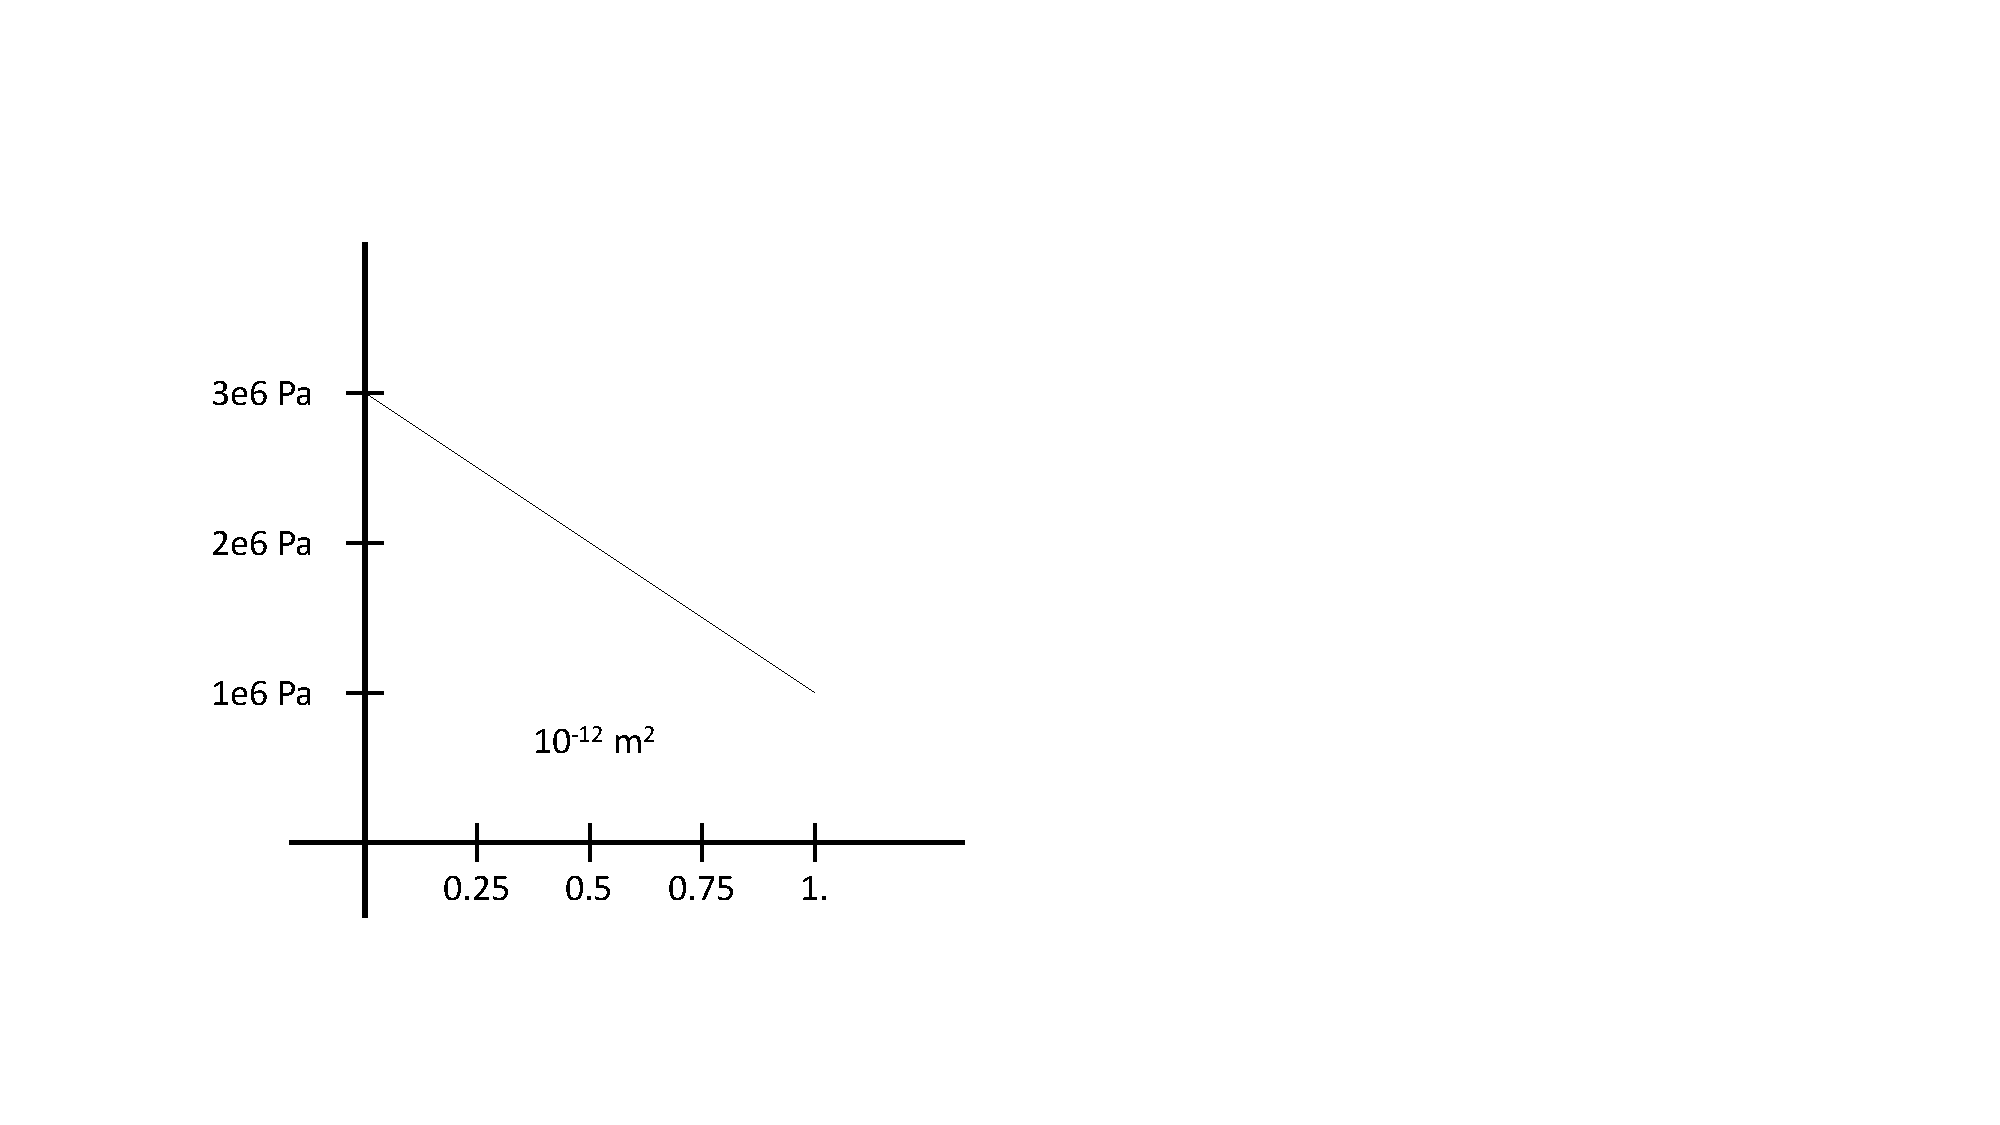
\includegraphics[width=0.8\linewidth]{figs/1d_uniform}
  \caption{Schematic of 1D uniform permeability problem.}
  \label{fig:1d_uniform}
\end{figure}

\newpage
\subsection{Block Permeability}
The 1D block permeability problem shown in Figure~\ref{fig:1d_block} has a permeability of $10^{-13}$ m$^2$ over the first half meter and $10^{-12}$ m$^2$ over the second half meter.
\begin{figure}[htbp]
  \centering
  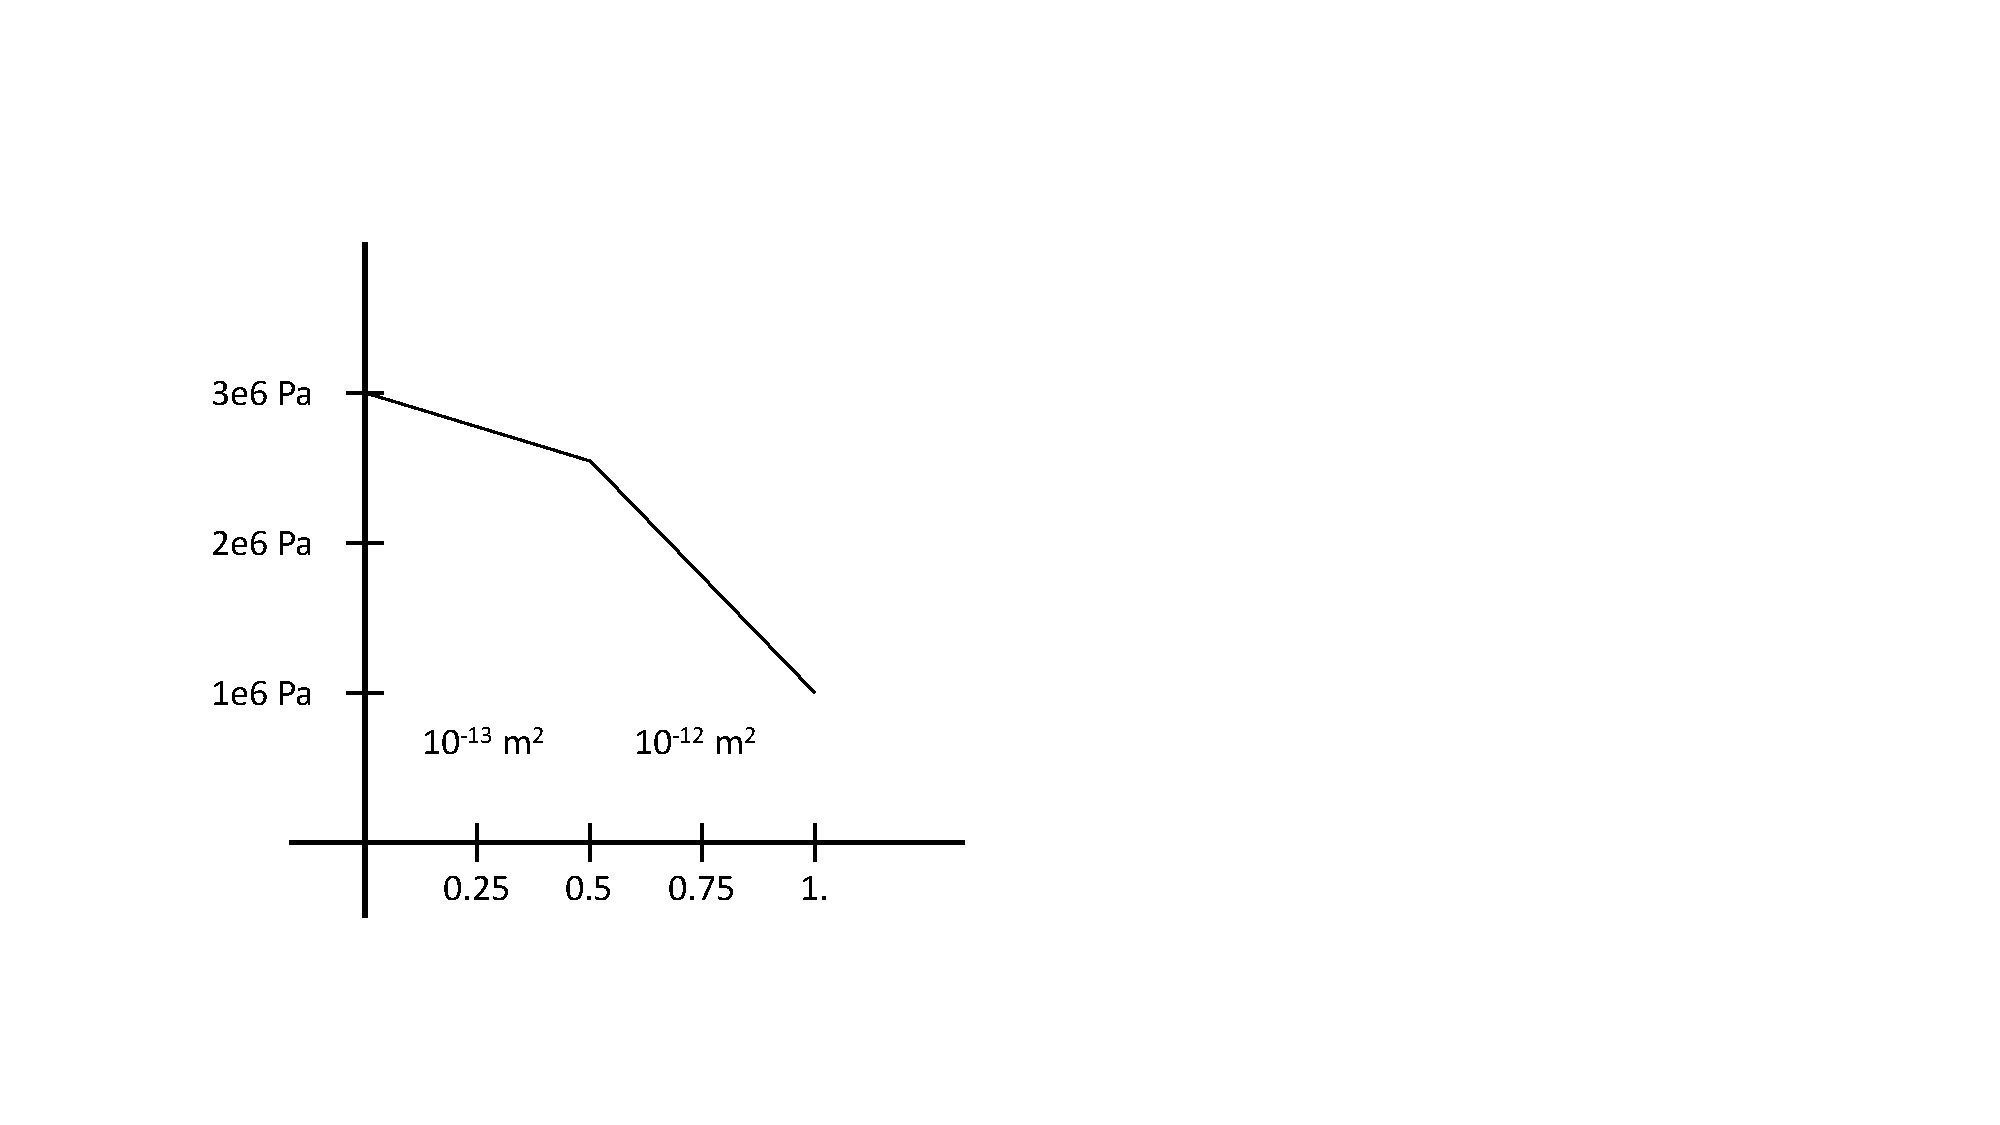
\includegraphics[width=0.8\linewidth]{figs/1d_block}
  \caption{Schematic of 1D block permeability problem.}
  \label{fig:1d_block}
\end{figure}

\newpage
\section{2D Pressure Field}
The 2D pressure field test problems consist of a 1$\times$1 meter square domain with Dirichlet (pressure) boundary conditions of $3\times 10^{6}$ Pa applied from <0,0-0.5> and <0-0.5,0> and $1\times 10^{6}$ Pa applied from <1,0.5-1> and <0.5-1,1>. 

\subsection{Uniform Permeability}
The 2D uniform permeability problem shown in Figure~\ref{fig:2d_uniform} has a uniform permeability of $10^{-12}$ m$^2$.
\begin{figure}[htbp]
  \centering
  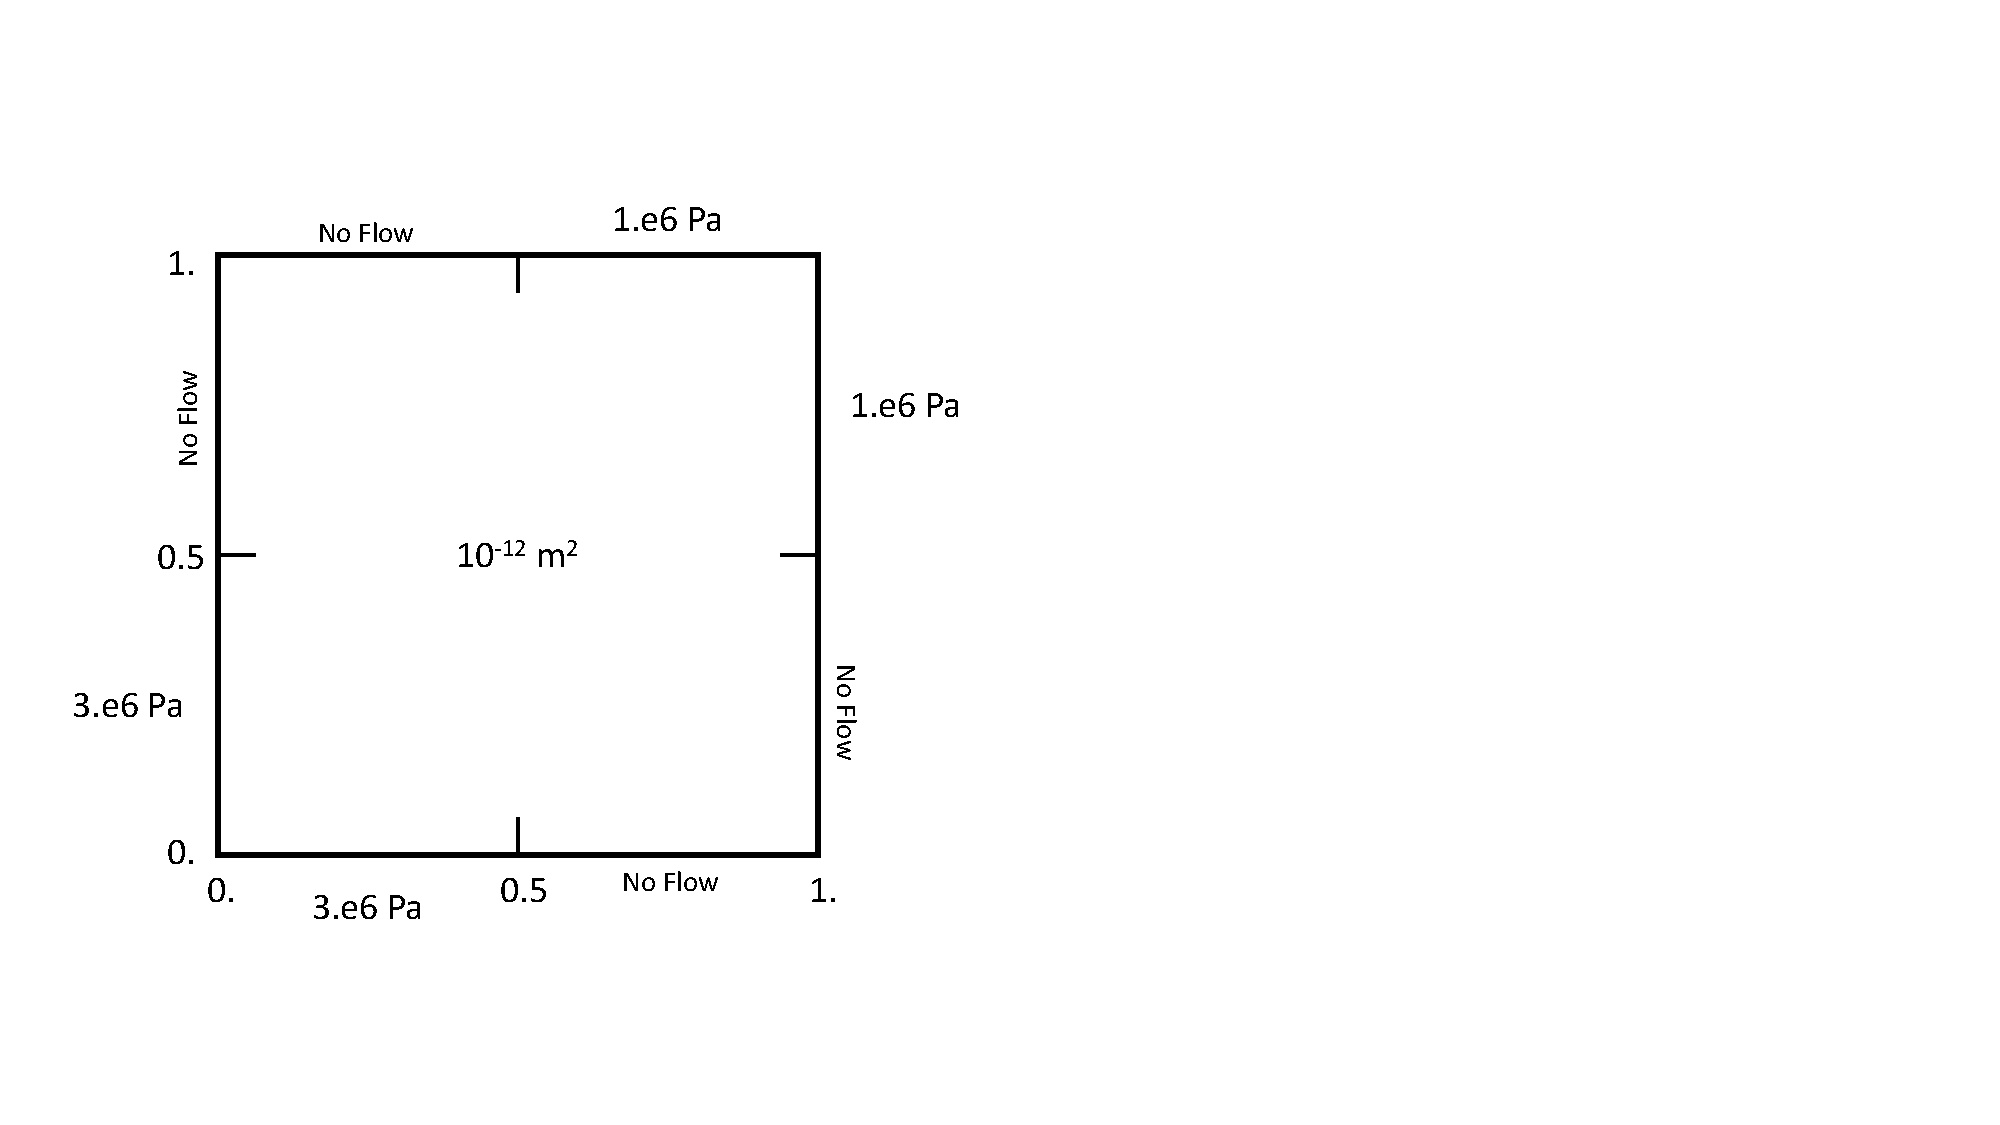
\includegraphics[width=0.9\linewidth]{figs/2d_uniform.pdf}
  \caption{Schematic of 2D uniform permeability problem.}
  \label{fig:2d_uniform}
\end{figure}

\newpage
\subsection{Block Permeability}
The 2D block permeability problem shown in Figure~\ref{fig:2d_block} has a permeability of $10^{-13}$ m$^2$ in the lower left and upper right quadrants and $10^{-12}$ m$^2$ in the upper left and lower right quadrants.
\begin{figure}[htbp]
  \centering
  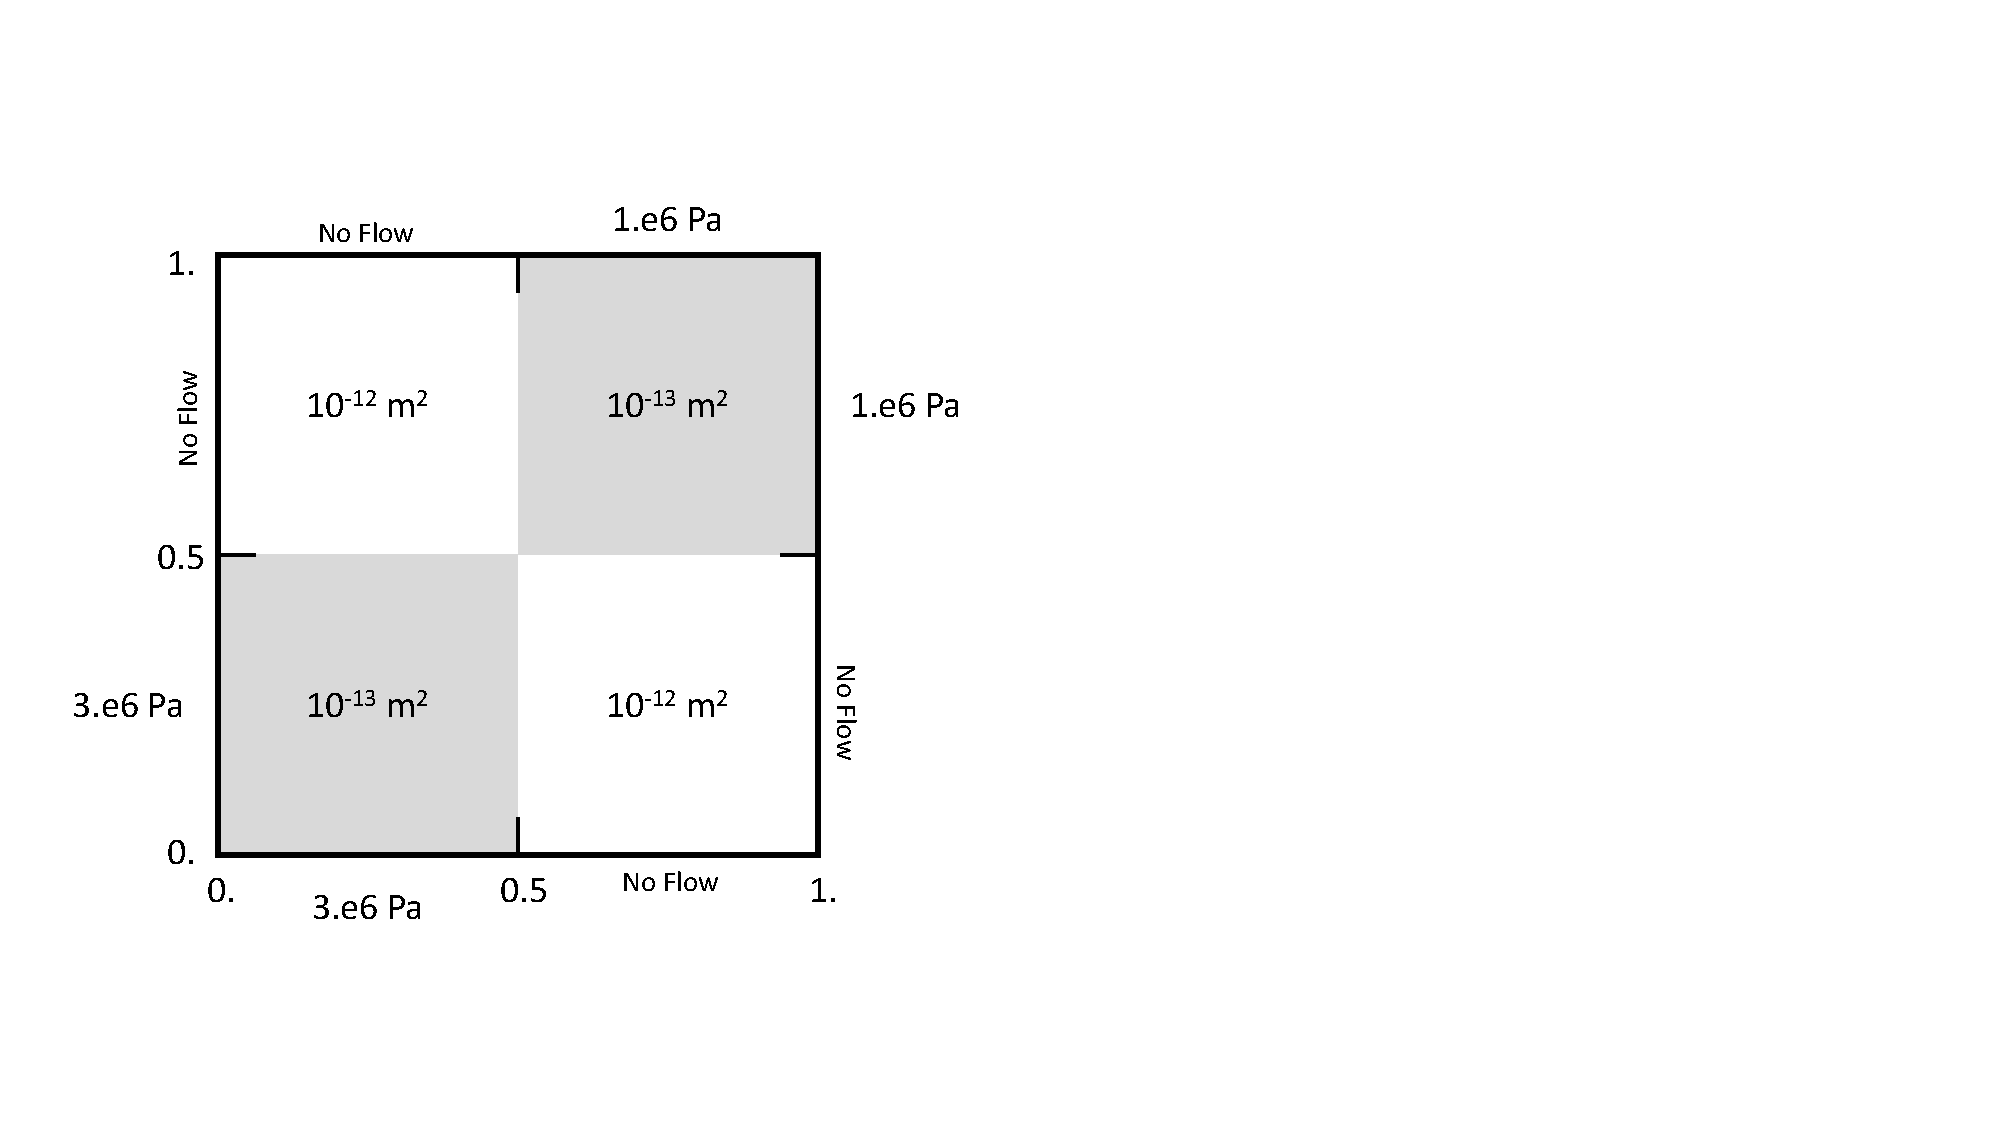
\includegraphics[width=0.9\linewidth]{figs/2d_block.pdf}
  \caption{Schematic of 2D block permeability problem.}
  \label{fig:2d_block}
\end{figure}

\newpage
\subsection{Block Permeability with Graded Pressure}
The 2D block permeability problem shown in Figure~\ref{fig:2d_block} has a permeability of $10^{-13}$ m$^2$ in the lower left and upper right quadrants and $10^{-12}$ m$^2$ in the upper left and lower right quadrants. The Dirichlet pressure boundary condition is assigned to all boundaries with a linear gradient between 3 MPa at the lower left corner and 1 MPa at the upper right corner, and 2 MPa at the opposite corners.
\begin{figure}[htbp]
  \centering
  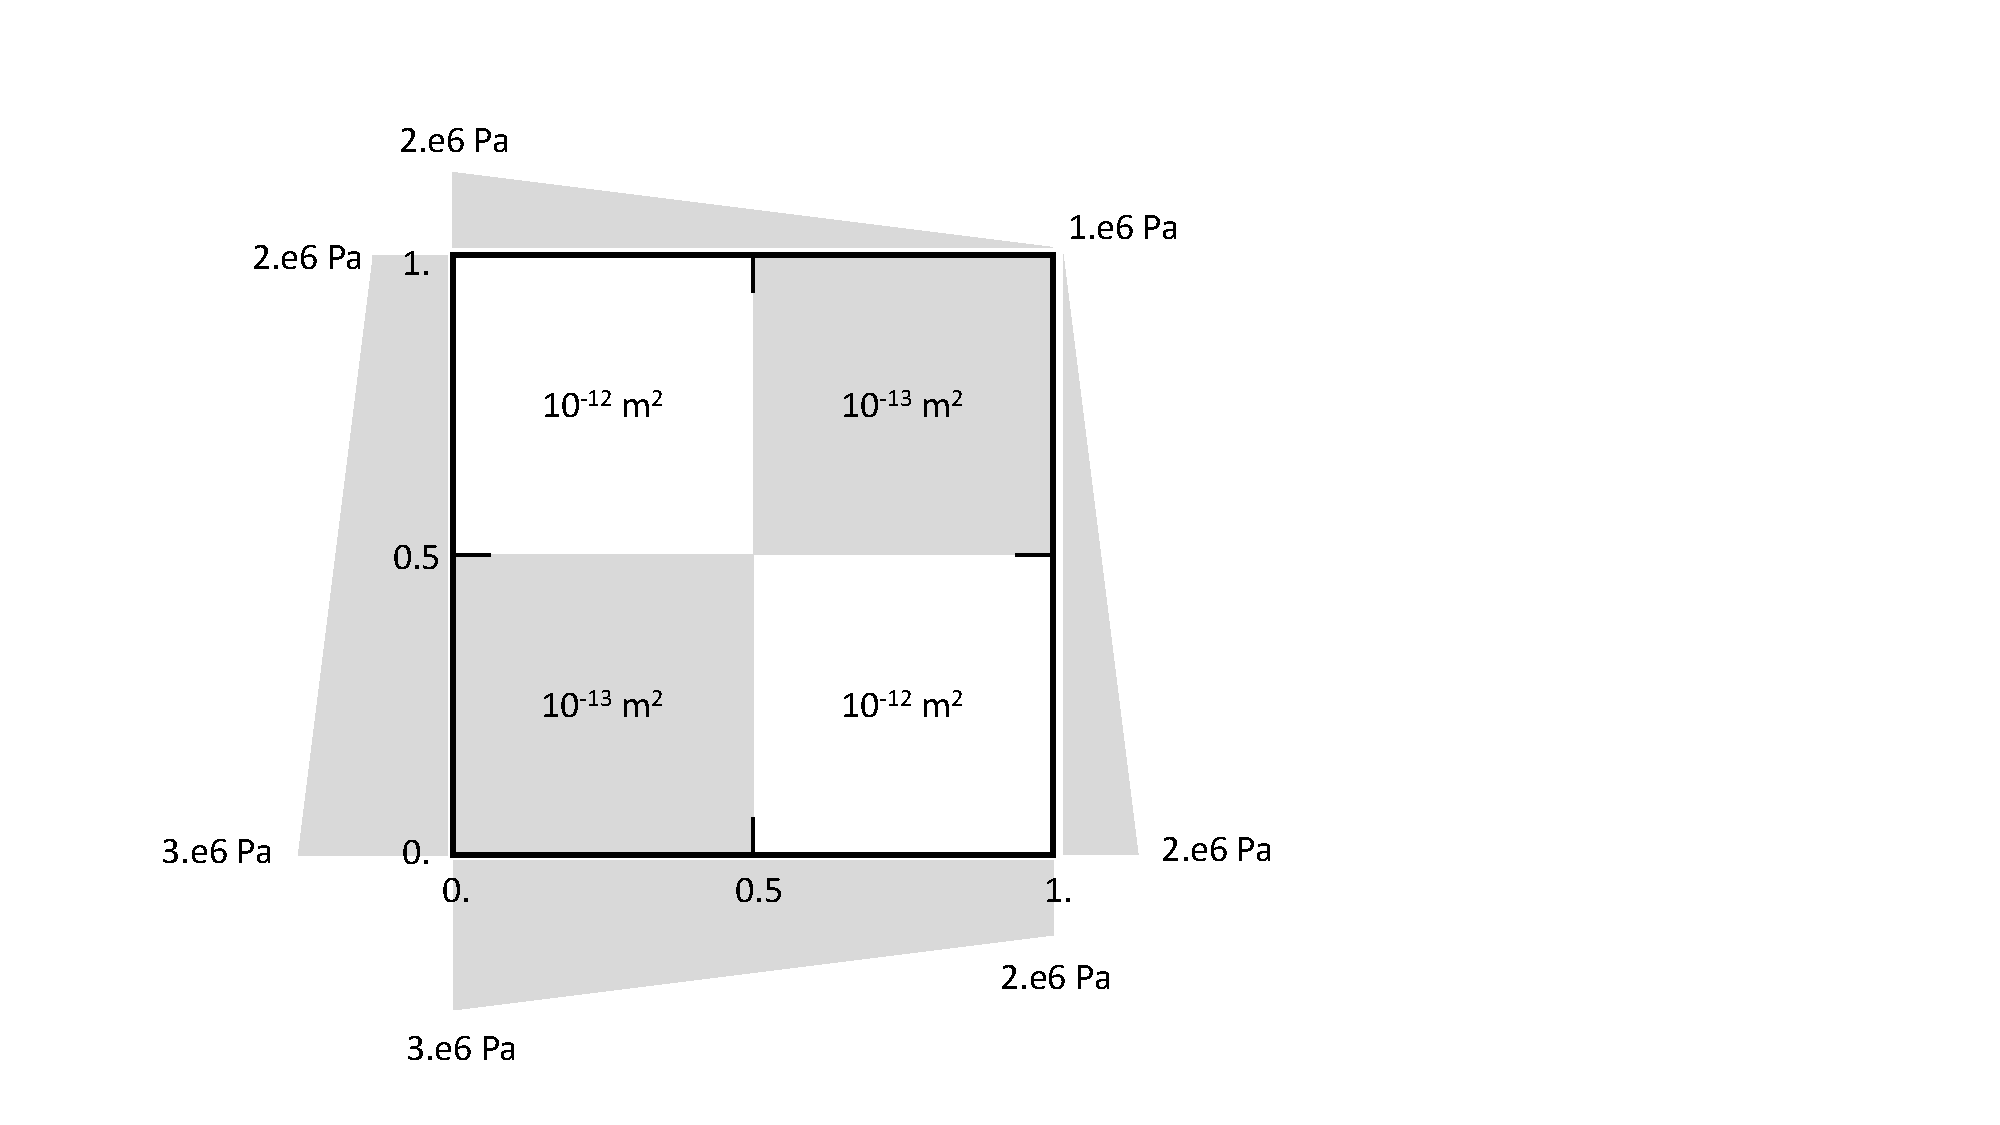
\includegraphics[width=0.9\linewidth]{figs/2d_block_graded.pdf}
  \caption{Schematic of 2D block permeability problem with a graded pressure boundary condition.}
  \label{fig:2d_block_graded}
\end{figure}

\end{document}

